\documentclass[12pt]{article}
\usepackage{tkz-tab}
\usepackage{tikz}
\usepackage{xcolor}
\usepackage{amsmath}

\begin{document}
\begin{center}
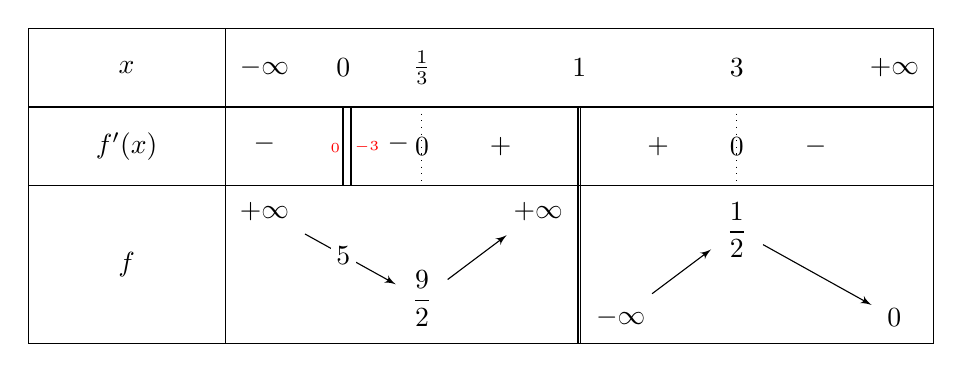
\begin{tikzpicture}
  \tkzTabInit[lgt=2.5, espcl=2]
    {$x$/1, $f'(x)$/1, $f$/2}
    {$-\infty$, $\frac{1}{3}$, $1$, $3$, $+\infty$}

  \tkzTabLine{ ,   , z , + , d , + , z , - }
  \tkzTabVar{+/$+\infty$ , -/ $\dfrac{9}{2}$ , +D-/$+\infty$/$-\infty$ , +/ $\dfrac{1}{2}$ , -/ $0$}
  \tkzTabVal{1}{2}{0.5}{$0$}{5}

  % Barres verticales à x = 0
  \draw[thick] (4.0, -2) -- ++(0, 1);
  \draw[thick] (4.1, -2) -- ++(0, 1);

	\node[above] at (3.9, -1.7) {\tiny\textcolor{red}{$0$}};
	\node[above] at (4.3, -1.7) {\tiny\textcolor{red}{$-3$}};

  	\node[above] at (3, -1.7) {\textcolor{black}{$-$}};
	\node[above] at (4.7, -1.7) {\textcolor{black}{$-$}};
\end{tikzpicture}
\end{center}

\begin{center}
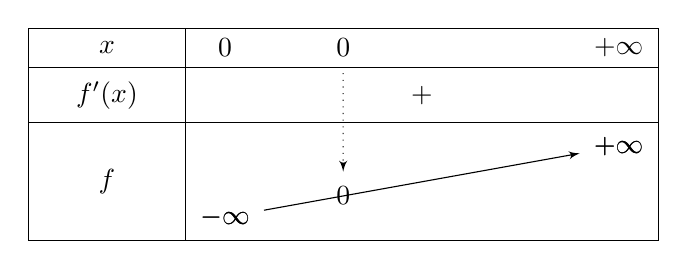
\begin{tikzpicture}[node style/.style={fill opacity=0,text opacity=1}]
        \tkzTabInit[espcl=5]{$x$/.5,$f'(x)$/.7,$f$/1.5}{$0$,$+\infty$}
        \tkzTabLine{,+,}
        \tkzTabVar{-/$-\infty$,+/$+\infty$/}
        \tkzTabVal[draw]{1}{2}{0.3}{$0$}{$0$}
\end{tikzpicture}
\end{center}

\begin{center}
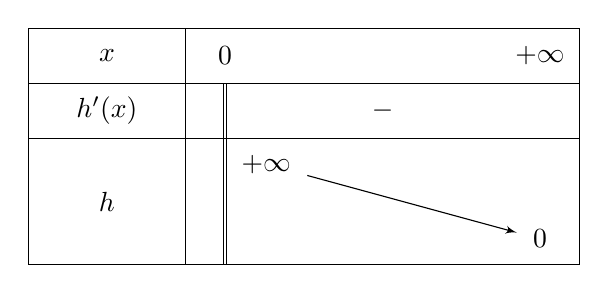
\begin{tikzpicture}
        % On définit l'initialisation du tableau : 
        % espcl=4 augmente l'espace horizontal pour que ce soit plus aéré.
        \tkzTabInit[espcl=4]{$x$ / .7 , $h'(x)$ / .7 , $h$ / 1.6}{$0$, $+\infty$}
        
        % La ligne de la dérivée : 
        % 'd' au début met la double barre en 0, puis on met le signe moins.
        \tkzTabLine{d, -, }
        
        % La ligne des variations de h :
        % D+ / $+\infty$ signifie : au niveau de la double barre (D), la limite est à gauche/haut (+).
        % - / $0$ signifie : la flèche descend (-) vers la valeur 0.
        \tkzTabVar{D+ / $+\infty$, - / $0$}
\end{tikzpicture}
\end{center}

\begin{center}
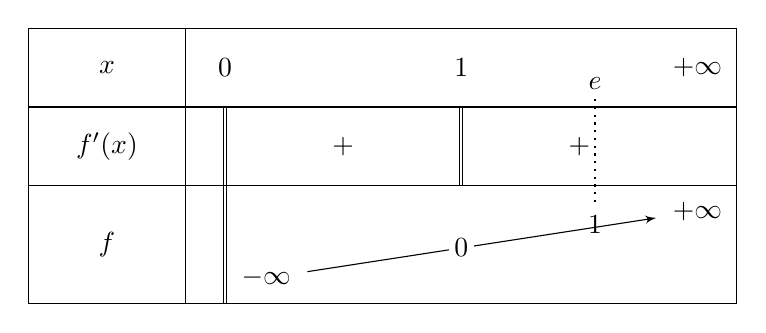
\begin{tikzpicture}
   \tkzTabInit{$x$ /1, $f'(x)$ /1, $f$ /1.5}
   {$0$ , $1$, $+\infty$}
   \tkzTabLine{d, +, d, +}
   \tkzTabVar{D-/$-\infty$, R/, +/$+\infty$}
   \tkzTabIma{1}{3}{2}{$0$}

\node (A) at (7.2,-0.7) {$e$};
\node (B) at (7.2,-2.5) {$1$};

\draw[dotted, thick] (A) -- (B);
\end{tikzpicture}
\end{center}

\end{document}